\apendice{Manual de especificación de diseño}

\section{Planos}
El montaje inicial, del que parte la idea de este proyecto con el objetivo principal de desarrollar un dispositivo completamente autónomo, se presenta en la Figura \ref{fig:arqInicio}.

\begin{figure}[h]
    \centering
    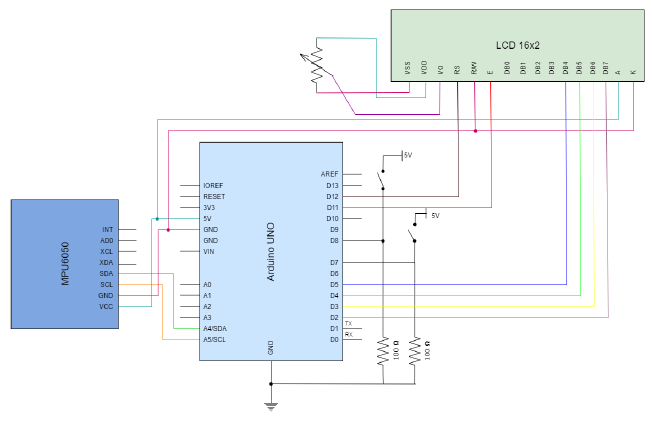
\includegraphics[width=1\textwidth]{img/E1_Planos/planoSara.png}
    \caption{Esquema de montaje del prototipo de partida. \cite{saragonz91:online}}
    \label{fig:arqInicio}
\end{figure}

Durante el trabajo se ha implementado una fuente de alimentación externa, regulada a través de un interruptor, y un módulo Bluetooth destinado a la transmisión de datos. La instalación del módulo HC-05 requiere únicamente cuatro conexiones: conectar Vcc al polo positivo, GND a toma de tierra, y las conexiones TXD (pin de transmisión) y RXD (pin de recepción) a los correspondientes opuestos en la placa Arduino, que en este caso se han configurado como los pines digitales 10 (RX) y 11 (TX). El montaje final se refleja en la Figura \ref{fig:arqFinal}.

\begin{figure}[h]
    \centering
    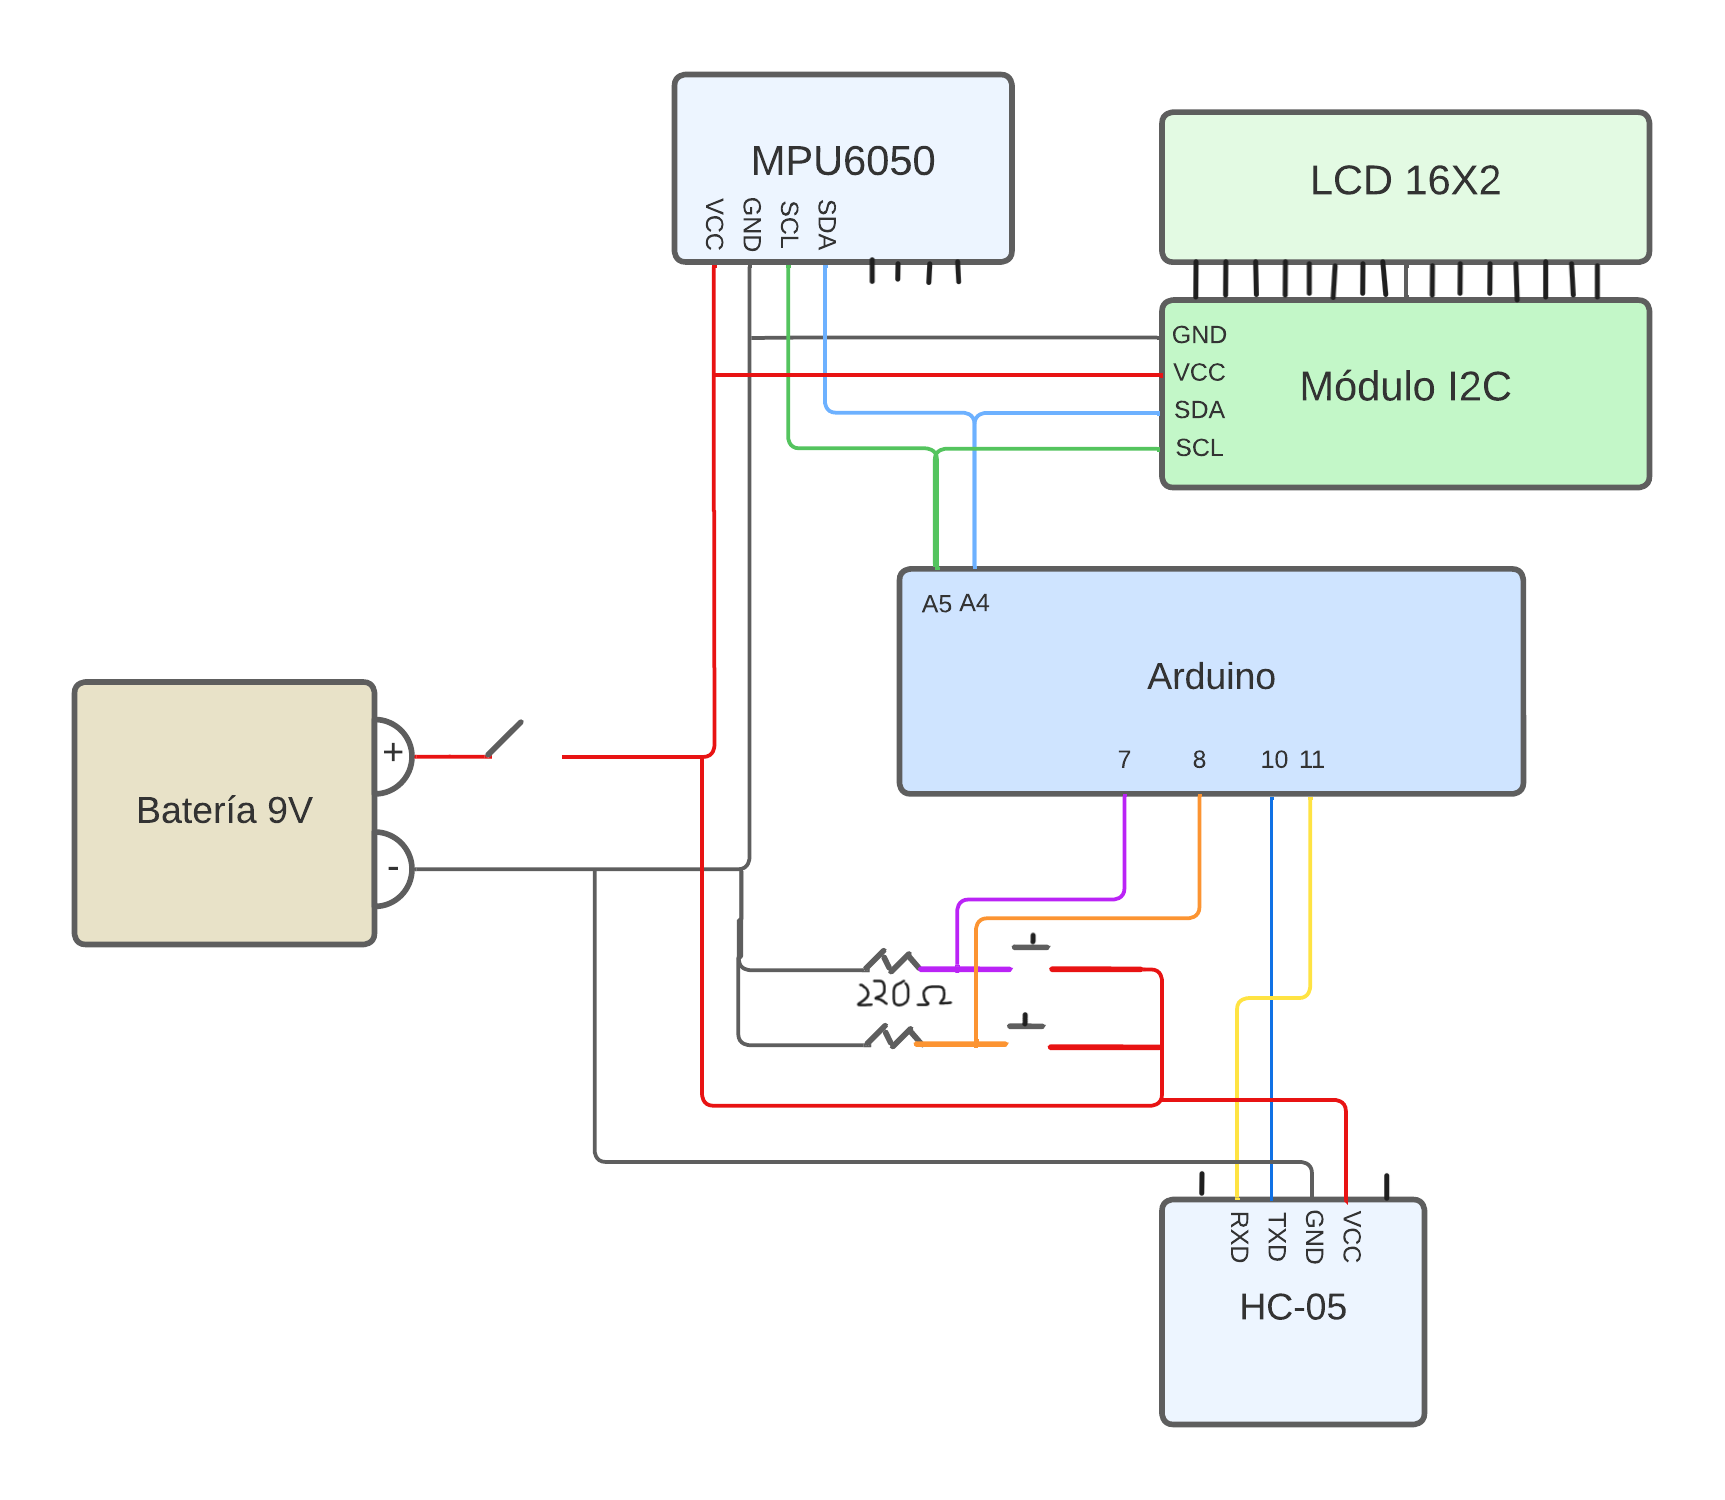
\includegraphics[width=1\textwidth]{img/E1_Planos/EsquemaArduino.png}
    \caption{Esquema de montaje del dispositivo final.}
    \label{fig:arqFinal}
\end{figure}

El protipo final, ilustrado en la Figura X, integra todos los componentes de hardware esenciales para facilitar su manejo.


\section{Diseño arquitectónico}
El diseño de la arquitectura web es el primer paso crítico en el diseño de software. Partiendo de los requisitos del sistema, el diseño arquitectónico proporciona una planificación y organización global de este, establenciendo las relaciones entre sus componentes \cite{castro2015arquitectura}.

Este proceso inicia con la obtención de los requisitos funcionales, detallados en el \textit{Anexo B.1}. Sin embargo, el paso esencial para la arquitectura web es el diseño de la experiencia de usuario. En este caso, se emplean diagramas de flujo que muestran las posibilidades del sistema para cada tipo de usuario.

Descripción del diagrama de flujo:
\begin{itemize}
    \item Figura \ref{fig:0_InicioFin}. Muestra el proceso de iniciar sesión en la página web y las opciones que comparten los usuarios en el menú. Redirige a otras figuras diferentes donde el diagrama de flujo continúa según el tipo de usuario que haya iniciado sesión.
    \item Figura \ref{fig:1_Admin}. Recorre las opciones presentadas al administrador en el sistema.
    \item Figura \ref{fig:2_Profesional}. Presenta el flujo de funcionalidades accesibles para el profesional y la relación entre ellas.
    \item Figura \ref{fig:3_Paciente}. Indica la forma de navegación del paciente en la web y la forma de acceder a cada acción posible.
\end{itemize}


\begin{figure}[h]
    \centering
    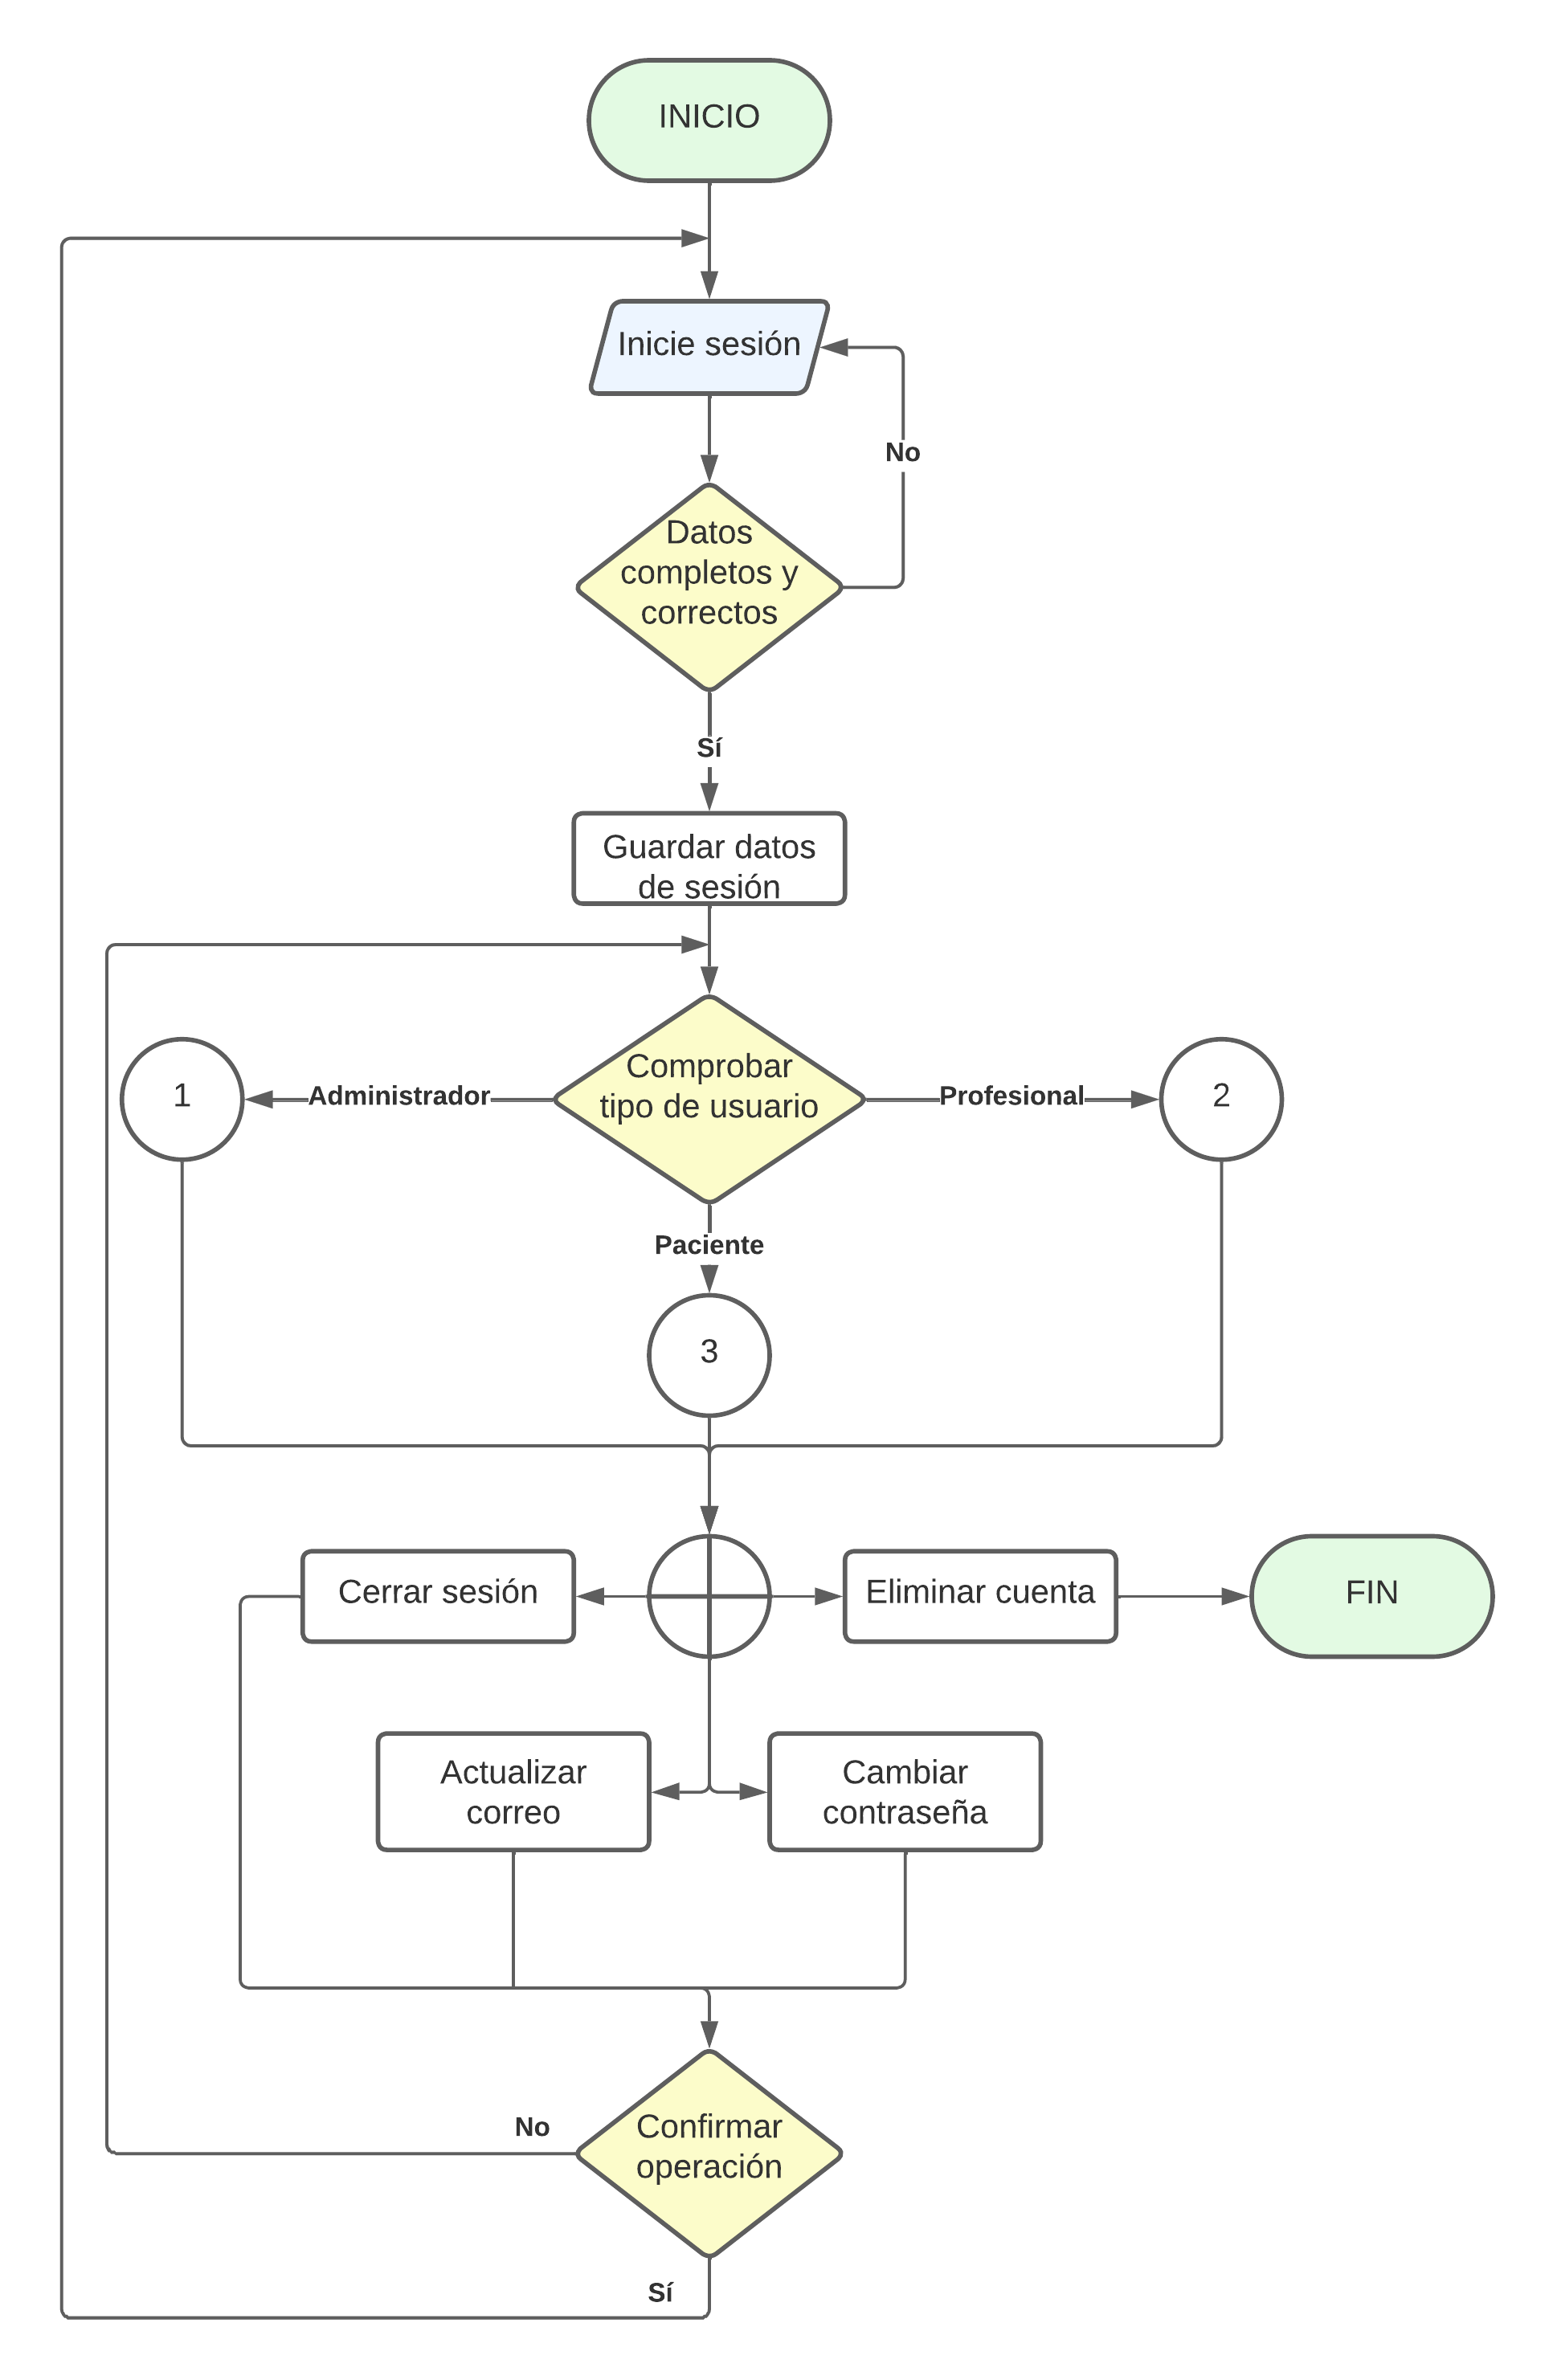
\includegraphics[width=1\textwidth]{img/E2_DiseñoArquitectonico/0_InicioFin.png}
    \caption{Diagrama de flujo - Inicio y fin de sesión.}
    \label{fig:0_InicioFin}
\end{figure}

\begin{figure}[h]
    \centering
    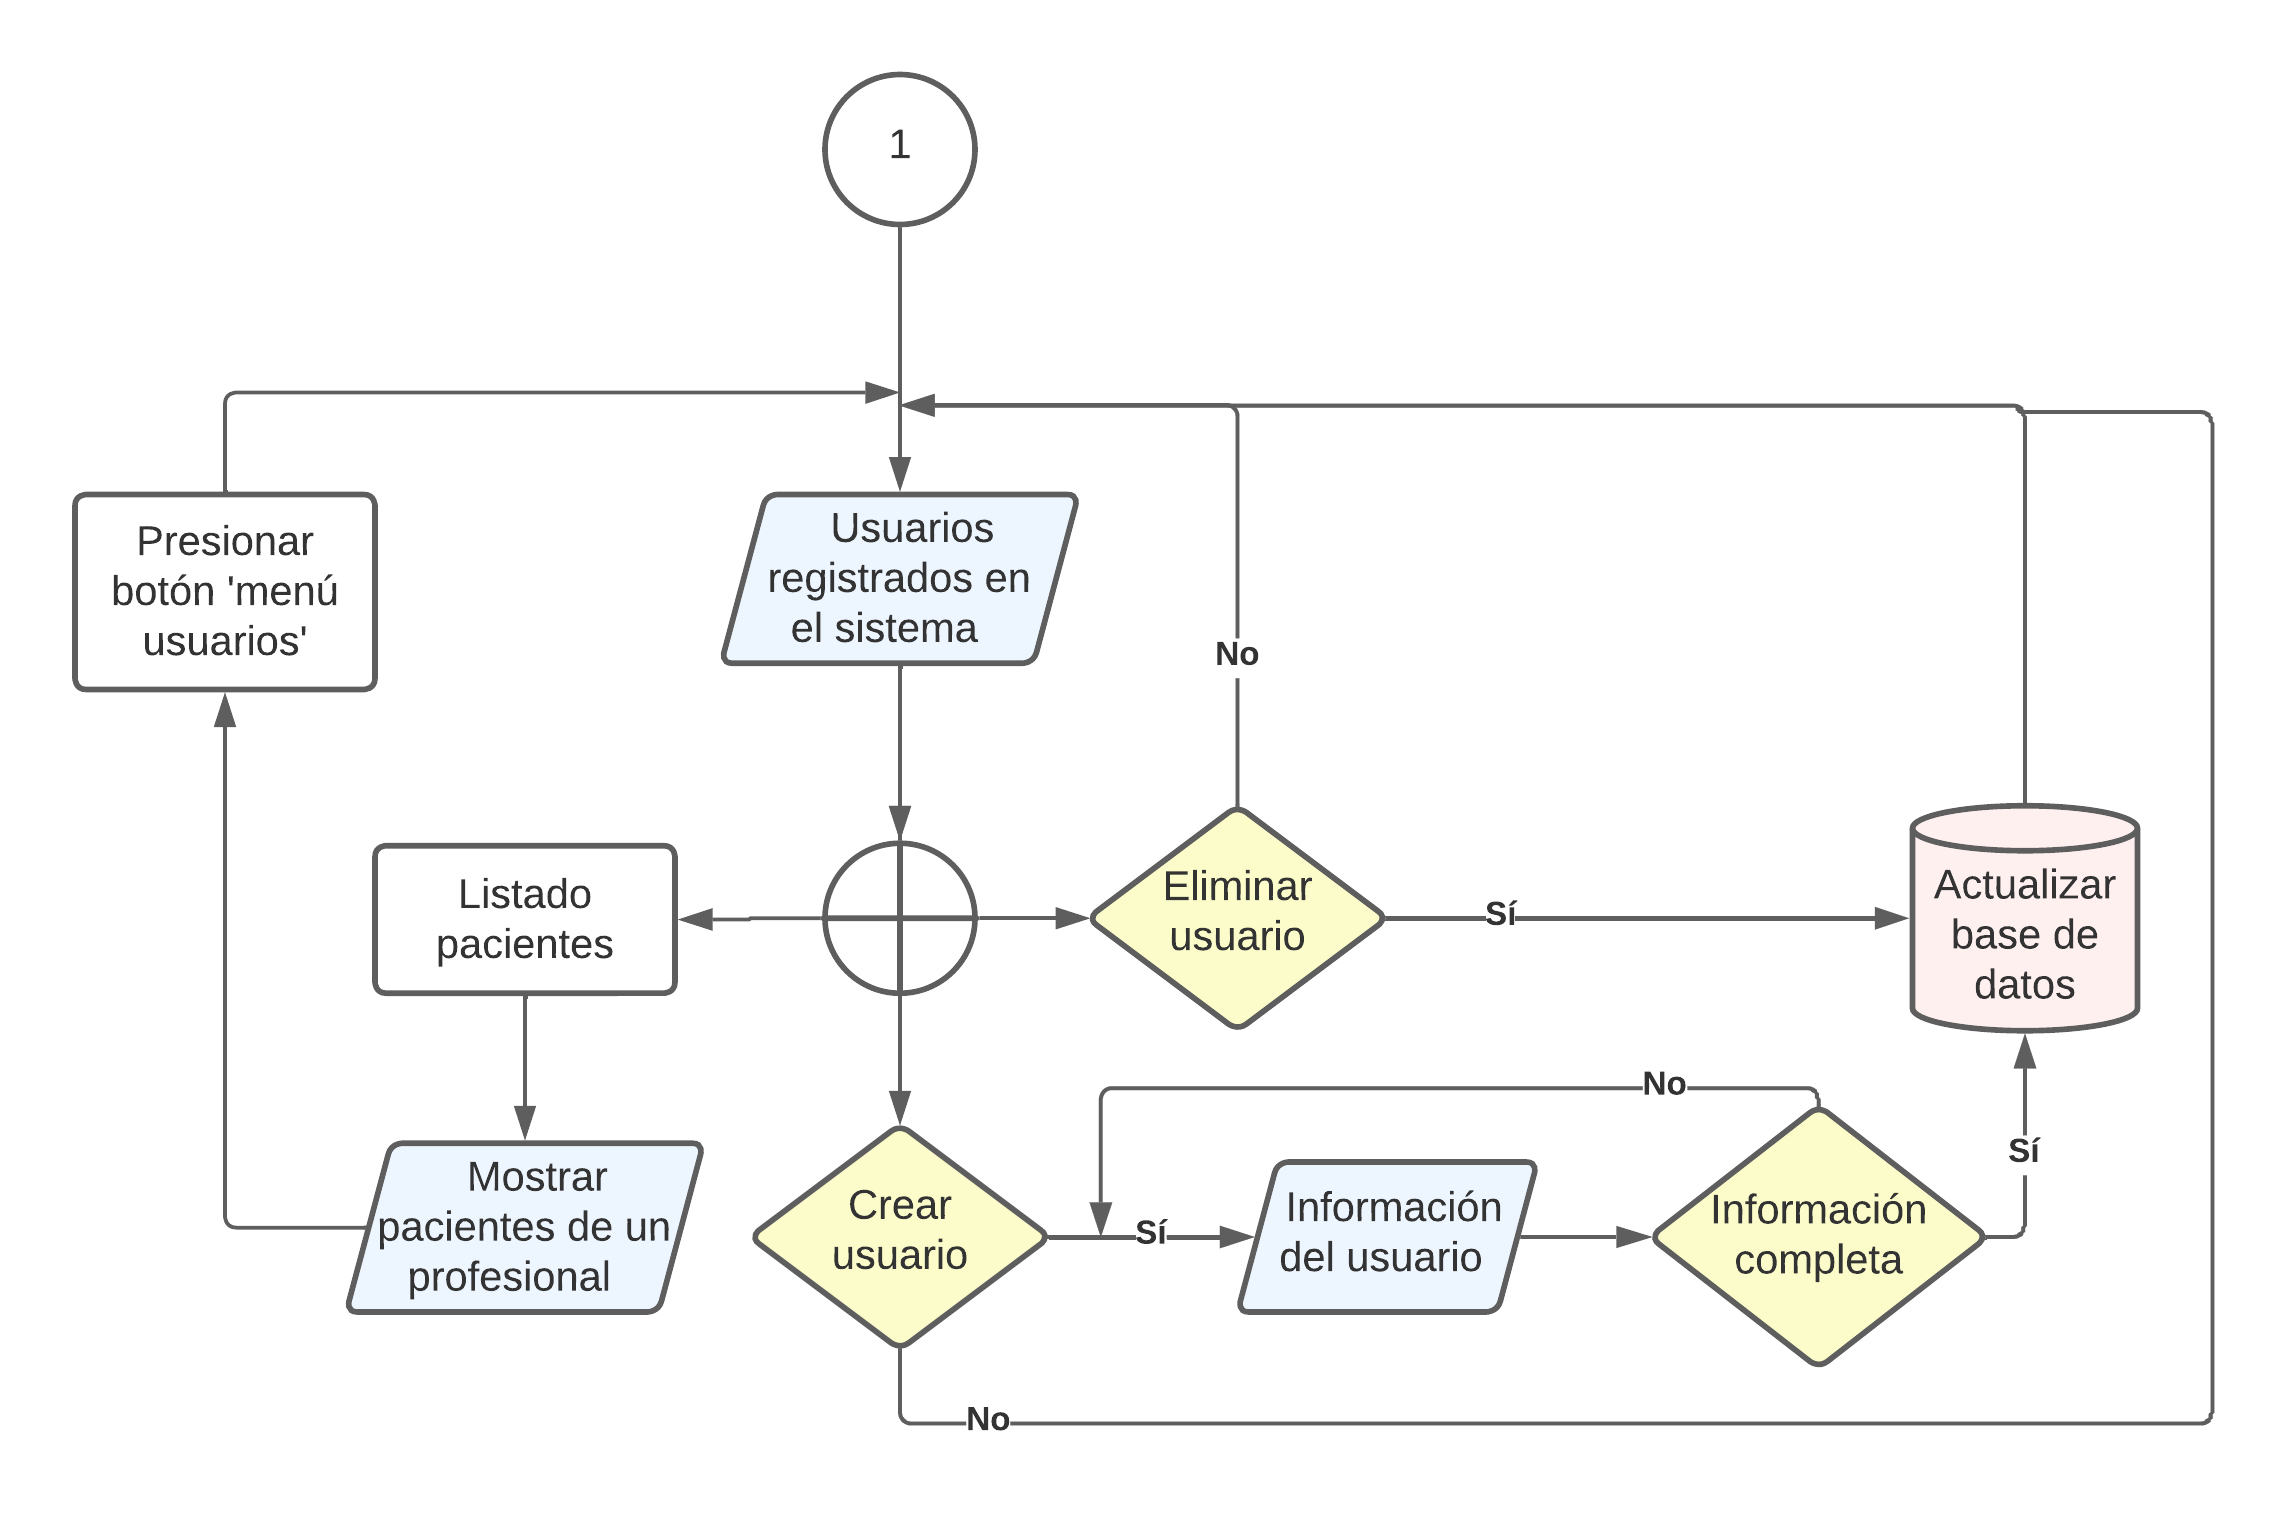
\includegraphics[width=1\textwidth]{img/E2_DiseñoArquitectonico/1_Admin.png}
    \caption{Diagrama de flujo. Usuario administrador.}
    \label{fig:1_Admin}
\end{figure}

\begin{figure}[h]
    \centering
    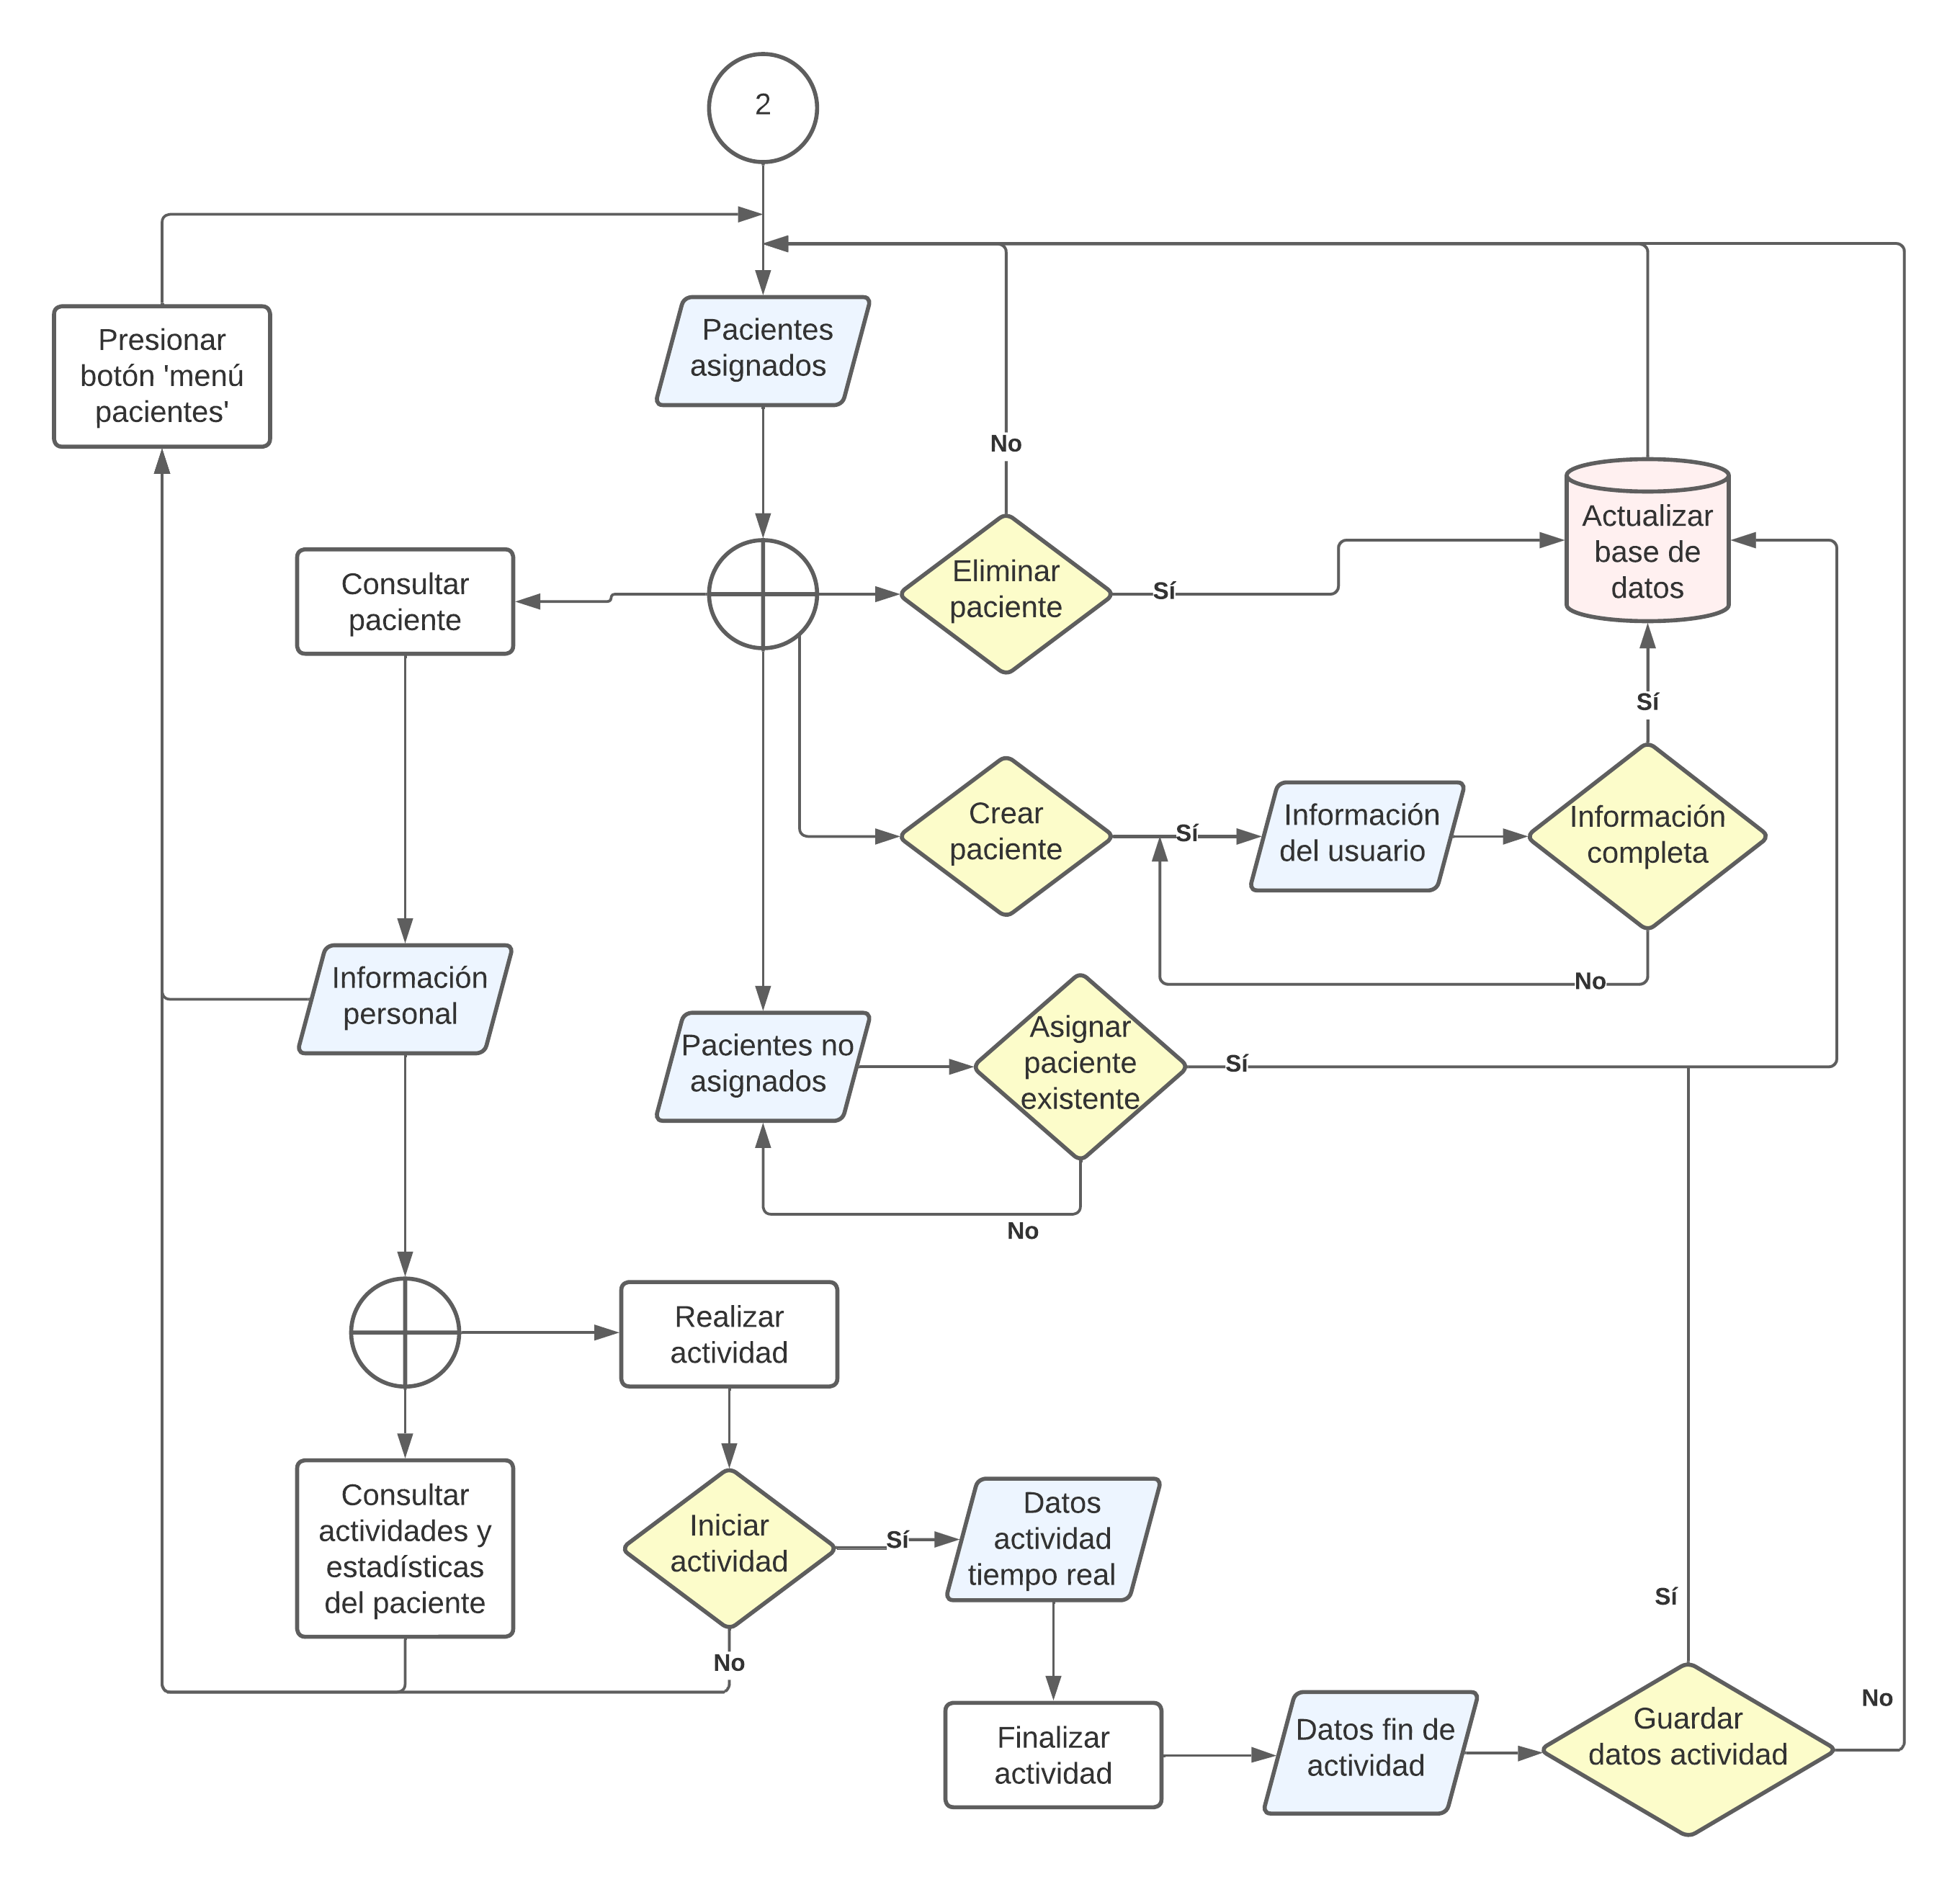
\includegraphics[width=1\textwidth]{img/E2_DiseñoArquitectonico/2_Profesional.png}
    \caption{Diagrama de flujo. Usuario profesional.}
    \label{fig:2_Profesional}
\end{figure}

\begin{figure}[h]
    \centering
    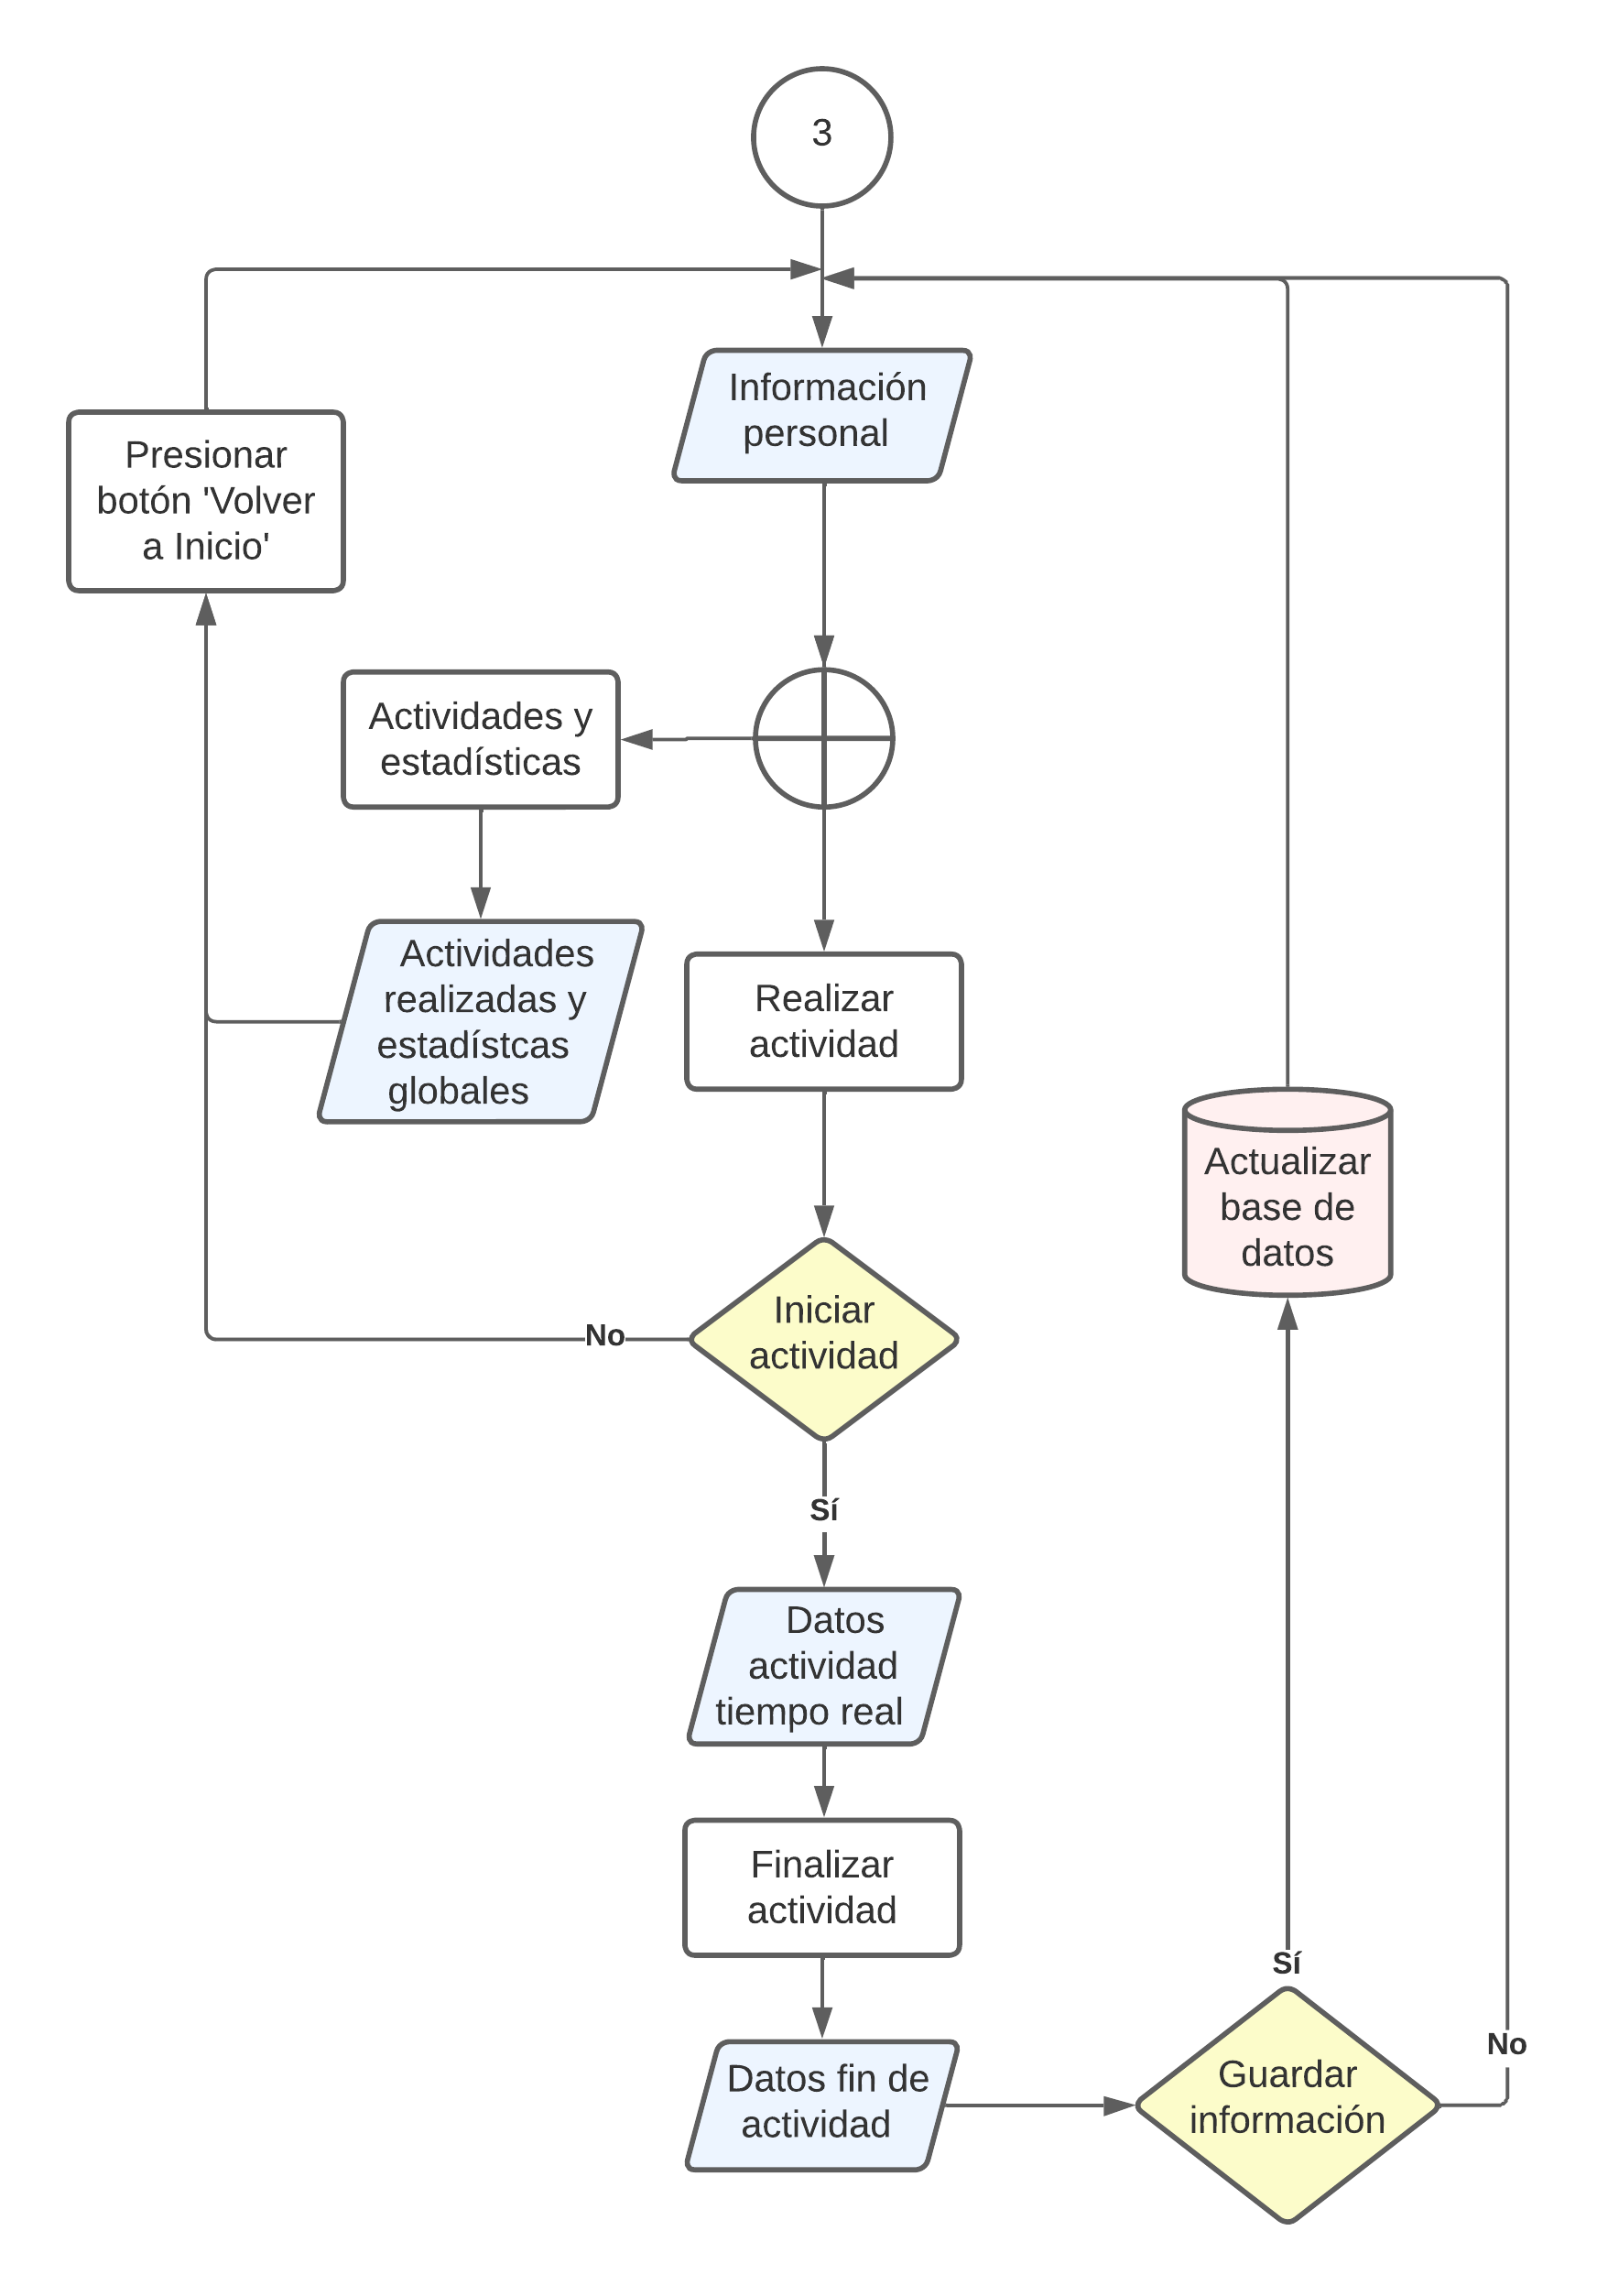
\includegraphics[width=1\textwidth]{img/E2_DiseñoArquitectonico/3_Paciente.png}
    \caption{Diagrama de flujo. Usuario paciente.}
    \label{fig:3_Paciente}
\end{figure}


En relación con el diseño de la interfaz de usuario, llevado a cabo mediante los wireframes que se presentan y describen en el \textit{Anexo F.3}, este se asocia principalmente con el desarrollo. Sin embargo, cabe destacar su alineación con la arquitectura web al establecer las pautas para la presentación de los elementos visuales.
